\documentclass[man,a4paper,12pt,floatsintext]{apa6}
\usepackage{apacite}
\usepackage{natbib}
\bibliographystyle{apacite}

\usepackage[american]{babel}
\usepackage{csquotes}
\usepackage{amsmath}
\usepackage{color,soul}
\DeclareUnicodeCharacter{2060}{\nolinebreak}
\usepackage{textgreek}
\usepackage{lscape}
\usepackage{hyperref}
\usepackage{wasysym} %inserir o símbolos 
\usepackage{booktabs}


\title{Hand differences in aiming task: analysis of dynamic brain networks with EEG}
\shorttitle{HAND DIFFERENCES IN AIMING TASK}

\fiveauthors{Lidiane Aparecida Fernandes}{Tércio Apolinário-Souza}{Gabriela Castellano}{Beatriz Couto Fortuna}{Guilherme Menezes Lage}
\fiveaffiliations{Universidade Federal de Juiz de Fora, Governador Valadares, Brazil}{Universidade Federal do Rio Grande do Sul, Porto Alegre, Brazil}{Universidade Estadual de Campinas, Campinas, Brazil}{Universidade Federal de Minas Gerais, Belo Horizonte, Brazil}{Universidade Federal de Minas Gerais, Belo Horizonte, Brazil}
\leftheader{Fernandes;Apolinário-Souza;Castellano;Fortuna;Lage}

\abstract {The studies explain the superiority of the right hand over the left through the shorter time spent in the feedback phase. This explanation makes sense for the temporal aspects of the task; however, there is a lack of explanations for the spatial aspects. This study investigates differences between the right and left hands in a goal-directed aiming task's pre-programming and feedback phases. The present study hypothesizes that the right hand is more associated with the feedback phase, while the left hand is more strongly associated with the pre-programming phase. Twenty-two participants performed 20 trials of the goal-directed aiming task with both hands. Overall, the results confirm the study's hypotheses. When analyzing the radial error, although the right hand stopped far from the target at the pre-programming phase, the right hand exhibited a lower radial error than the left hand. These findings imply that during the visual feedback phase, the right hand compensates for the higher error observed in the pre-programming phase, using the visual feedback to approach the target more closely than the left hand. Conversely, the left hand displayed a lower error at the pre-programming phase than the right, indicating a stronger association with the pre-programming phase.}

\keywords{Handedness, Manual Asymmetries, Motor Control}

\authornote{Correspondence concerning this article should be addressed to Tércio Apolinário-Souza, address: R. Felizardo, 750 - Jardim Botânico, Porto Alegre - RS, Brasil; CEP: 90690-200; E-mail: edf.tercio@gmail.com; ORCID: www.orcid.org/0000-0002-2136-0238; ResearcherID: O-7470-2016}

\begin{document}
\maketitle



\begin{flushleft}
\textbf{1. Introduction}
\end{flushleft}

Woodworth (1899), in a seminal article, demonstrated that manual goal-directed aiming is more accurate when performed with the right hand than the left. With the advancement of technology has furthered these findings using kinematics measures of movement \citep{Elliott2000}. The peak velocity, one of these kinematics measures, has been employed to explore the relative significance of central planning preceding movement initiation (pre-programmed phase or open-loop component of the movement) and the corrective processes that depend on the availability of feedback produced by the response (feedback phase or closed-loop component of the movement) \citep{Elliott2001b}. While the time interval before peak velocity reflects the pre-programmed characteristics of the movement \citep{Carlton1992}, the time interval after peak velocity indicates the visual error correction feedback required for accurate target attainment \citep{Elliott2010d}. 

Overall, the right hand tends to exhibit a longer duration to reach peak velocity compared to the left hand \citep{Mieschke2001b,Elliott1996}. This increase of time to peak velocity decreases, proportionally, the time available to make corrections through visual feedback \citep{Elliott1999a}. Several studies have shown these results \citep{Lavrysen2007,Lavrysen2012b,Roy1994,Buekers2000,Fernandes2022a}.	These results have been attributed to the higher efficiency of the right-hand/left hemisphere system in processing feedback \citep{Flowers1975a,Todor1978}. The defenders of this logic assume a shorter time making corrections in response to feedback reflects a higher efficiency of the system in processing feedback \citep{Cohen1973,Halperin1973}. In fact, the adjustments in response-produced feedback spend time, resulting in decreases in performance in temporal aspects of the task (ex., movement time)\citep{Meyer1988}. Because they spend time modulating the muscular forces used to propel and brake the movement \citep{Elliott2001b}. However, this explanation can reasonably to the superiority of the right hand over the left hand in the temporal aspect of the task, but not spatial. In other words, the accuracy of the right compared left hand,  be explained by the higher efficiency of the right-hand/left hemisphere system in processing feedback? 

Apolinário-Souza et al. (2023) examined these questions using measures that split the spatial accuracy of the pre-programmed phase and the spatial accuracy of the feedback phase. The relation between radial error at the moment of peak velocity and radial error end movement was used to get the spatial accuracy of the pre-programmed and feedback phases. The results indicated that the right hand made more radial errors at the moment of peak velocity than the left hand, indicating that the pre-programmed phase of the left hand was better in spacial terms. In contrast, the right hand generated less radial error in the second movement phase (feedback phase) than the left. The authors speculated that the right made corrections with visual feedback more efficiently because, although it had stopped more distant in the first moment (pre-programmed phase), get closer to the target in the second moment (feedback phase). However, the authors did not use measures to infer efficiency in corrections. 

One way to infer efficiency in corrections is by using measures to capture the relation between the number of corrections and the radial errors of the feedback phase. The number of corrections can indicate the tries of the system to correct the movement by visual feedback, commonly measuring the number of zero crossings in the acceleration profile (number of discontinuities)\citep{Elliott2010d}. The radial errors of the feedback phase can be obtained from the discrepancies between the radial error at peak velocity and the radial error of end movement. If the right hand makes fewer corrections but has more radial errors in the feedback phase than the left hand, this could indicate greater efficiency in corrections. Because, for a minor number of corrections, more errors were corrected. This same logic can be attributed to the time spent in the feedback phase. More corrections within a shorter available time, greater efficiency are considered. Because, the modulation of the muscular forces used to propel and brake the movement was adequate to the extent that it did not consume time. Another approach to infer efficiency in corrections is through the utilization of the area under the curve generated by corrections over time. This metric provides insights into the magnitude and duration devoted to corrections. An expanded area under the curve could imply corrections characterized by greater magnitude and longer duration.


Figure 1 summarizes the four novel measures proposed to infer efficiency in corrections. Figure 1 shows that both hands produced the same number of corrections (indicated by ND), but the error of the right hand was minor. This indicates that with a lower of units of the number of corrections, the right hand reduced the error more. Figure 2B demonstrates that both hands produced equal corrections, but the right hand spent less time (proportionally) than the left hand in the second moment (feedback phase). Additionally, in Figure 2B, the area under the curve for the first submovement is smaller for the left hand than for the right hand. Conversely, the area under the curve for the second submovement of the right hand is smaller than that of the left hand.

\begin{center}
\textbf{[Insert Figure 1 here]}
\end{center}

Considering Apolinário-Souza et al. (2023), we hypothesize that the right hand will show more efficiently in corrections than the left hand. Furthermore, we sought to replicate the finds of Apolinário-Souza et al. (2023) in relation pre-programming and feedback phases of a goal-directed aiming task. Thus, the present study investigates differences between hands in the pre-programming and feedback phases of a goal-directed aiming task.




	

\begin{flushleft}
\textbf{2. Methods}
\end{flushleft}
\subsection{2.1 Participants}
Twenty-two undergraduate students, male, ranged in age from 18 to 35 years old (mean = 24.7, standard deviation = 5.61) as participants in this experiment. We estimated the required sample size by power analysis using r  \url{(http://cran.r-project.org/web/packages/pwr/)}. We assumed an alpha of 5\%, an effect size of 0.50, and a power of 0.90. The analysis suggested a sample size of 21.9 participants for paired t-test (paired t-test). All participants were right-handed university students whose mean laterality quotient on the Edinburgh Handedness Inventory (Oldfield, 1971) was 91.7. All participants had normal or corrected-to-normal visual acuity in both eyes. The volunteers had no prior experience with the experimental task.

A local ethics committee approved the study (CAAE: 02437218.3.0000.5149 ). All participants provided written informed consent after receiving a full explanation of the study. 
	
\subsection{2.2 Apparatus and Task}

A goal-directed aiming task was administered in previous studies \citep{Fernandes2018c,Fernandes2022a,Lage2012c,Lage2013b,Oliveira2019}. The motor task involved moving a non-inking pen on a digitizing tablet in such a way that the cursor on the computer screen would move from an initial point (subject's midline) to a target located 21 cm away at a 45° angle from the starting position. The target had a diameter of 0.5 cm and was positioned on either the right or left side, resulting in a difficulty index of 6.2 bits \citep{Fitts1958}. We used a non-inking pen with a Wacom Intuos 3 digitizing tablet (30.4 cm  30.4 cm, RMS accuracy 0.01 cm). The tablet was attached to the computer with a 32-inch monitor, running the customized software (free access \url{https://github.com/apolinario-souza/APONTAMENTO/tree/master/Linger}). The distance traveled by the non-inking pen on the tablet was proportional to the distance traveled by the cursor on the computer screen.

\begin{center}
\textbf{[Insert Figure 2 here]}
\end{center}


Te B-Alert×10 sensor headset (Advanced Brain Monitoring Inc., Carlsbad, CA, USA) was used to acquire the electroencephalography (EEG). Nine Ag/AgCl EEG electrodes were located at F3, Fz, F4, C3, Cz, C4, P3, POz, and P4, according to the international 10–20 system. Two electrodes on the mastoid bones (lef and right) were used as the reference and ground. Te sampling rate was 1,024 samples/s for all channels and transferred in real-time via Bluetooth link to a host computer where the B-Alert sofware (Advanced Brain Monitoring Inc., Carlsbad, CA) stored. All electrode impedances were maintained below 5 k$\Omega$.  


The motor task was developed using LabVIEW software (National Instruments, Texas, USA). The processing, storage, and data filtering of the motor task were also implemented in LabVIEW (National Instruments, Texas, USA). The data obtained during the motor task were acquired at 200 Hz and filtered using a second-order Butterworth low-pass filter with a cutoff frequency of 12 Hz. The criterion for the start and end of the movement relied on a zero rate of position change for 80 milliseconds (ms). If the position (x-axis and y-axis) did not vary within an 80 ms time window, the participant's manipulated non-inking pen was assumed to be stationary. 

\subsection{2.3 Procedures and Experimental Design}
	
We conducted the data in a dedicated room specifically designated for this purpose. Participants began by signing the informed consent form and completing the Edinburgh Handedness Inventory \citep{Oldfield1971a}. Falar do posicionamento do EEG. 


Subsequently, they were briefed on the experimental procedures and received standardized verbal instructions: "Strive to execute the movement the fastest and precision possible, concluding the motion within the target area".

Participants performed three practice trials to familiarize themselves with the motor task, exclusively using their starting hand. These three practice trials, familiarization trials, ensured that the participant understood the intended movement and did not use it for analysis. Immediately after, the participants performed 20 trials of the motor task with each hand in a counterbalanced manner. Namely, half of the participants started with their right hand, and the other half started with their left hand.

Participants placed the pen on the digitizing tablet at the corresponding position to the starting point (home position). Upon correct positioning at the starting point, participants were immediately given an auditory signal (a 700 Hz tone lasting 200ms) indicating the correct position. We instructed the participants to wait to move the pen until the trial started signal. We fixed the starting point and positioned the targets on the right side for the task performed with the right hand and on the left side for the task performed with the left hand. After a 1-second interval, the warning stimulus was presented. This stimulus entailed the removal of the initial point and target on the monitor screen, resulting in a blank screen. Subsequently, within a randomly assigned timeframe ranging from 2 to 3 seconds, participants were presented with a visual and auditory stimulus (consisting of a 200 ms duration 500 Hz tone), indicating the commencement of the movement (imperative stimulus). The imperative stimulus marking the start of the movement involved the reappearance of the initial point and target on the monitor screen. Upon completing the movement, participants were instructed to lift the pen from the digitizing tablet and reposition it for the subsequent attempt without sliding it across the table. The participant had a maximum of 1.5 seconds to complete the trial.

\begin{center}
\textbf{[Insert Figure 3 here]}
\end{center}

\subsection{2.4 EEG signal processing}
The 60 Hz notch filter was applied in the signal. Then, the zero-phase pass-band filter (lower cutoff of 0.1 Hz and an upper cutoff of 100 Hz) and the zero-phase high-passed filter (lower cutoff of 1 Hz) applied in the signal to remove the DC offset. Finally, the multidimensional median filter was used with a window size of 10 ms.

Subsequently, all electrodes were filtered in the interest bands using a finite impulse response (FIR) filter using the window method. The bands were, theta (4–7 Hz), alpha lower (8–10 Hz), and alpha upper (10–12 Hz).

After the EEG signals were filtered in the interest bands and computed the phase value using the Hilbert transform, the signals were epoched in three moments: (1) planning - the interval between the sign for initiation of trial and key press 2; (2) execution -  the interval between pressing keys 2 and 4; (3) processing - the interval between key press 4 and the sign for initiation of the subsequent trial. Data from the motor task and EEG were synchronized offline by an algorithm developed in Python (https://osf.io/q8yjp/). Details of offline synchronization can be seen in Nogueira et al. (2020).  

	
\subsection{2.5 Measurements}

The performances examined were reaction time, movement time, radial error, and angle error. The reaction time (RT) was the time from the beginning of the imperative stimulus until the beginning of the stroke. Movement time (MT) encompasses the time interval between the initiation and finish of the movement. We obtained the radial error (RE) through the following equation:
\[ 
RE(i) = \sqrt{(x_i-x_t)^2+(y_i-y_t)^2} 
\]

where $x_i$ and $y_i$ are the values of the final position produced in the x and y-axis performed in each trial, and the $x_t$ and $y_t$ are the target positions. The angle error (AE) was obtained through the following equation:
\[ 
a_\theta (i) = \dfrac{x_i}{\sqrt{(y_i^2+x_i^2)}}
\]
\[
a(i) = (\dfrac{arcsin(a_\theta(i))}{\pi})*180 
\]
\[
AE (i) = |a_i-45|
\]

where $x_i$ and $y_i$ are the values of the final position produced in the x and y-axis performed in each trial,  the $a_\theta (i)$ and $a(i)$ are values of angle, in radians and degrees, respectively, of the final position produced. We used the value of 45 degrees, the straight line angle between the target and the starting position (home position). 

To address the question regarding about pre-programming phase and feedback phase, the movement was divided into primary and secondary submovements by identifying the first negative-to-positive zero crossing observed after the absolute peak velocity in the acceleration profile. The primary submovement corresponds to the initial segment of the movement, representing the preprogrammed phase. In contrast, the secondary submovement represents the feedback phase \citep{Elliott2010d}. The relative time to peak velocity (RTPV) is a measure that divides the movement into two phases, which are related to the timing of the primary submovement or preprogrammed phase. The larger this measure, the longer the duration of the first submovement \citep{Lage2013b}. In the secondary submovement, the number of zero crossings in the acceleration profile is accounted for in the measure of the number of discontinuities (ND). This measure reflects online movement trajectory adjustments based on feedback about movement errors. Peak velocity (PV) is the maximum velocity value attained during the movement trajectory toward the target. This measure enables inferences regarding disparities in the force modulation produced by the limb during the initial impulse phase \citep{Lage2014b}. 

Researchers have commonly utilized PV, RTPV, and ND metrics to infer motor control in the goal-directed aiming task (see Elliott et al., 2010 for a review). Likewise Apolinário-Souza et al.,XXX, this study including radial error and angle error at the end of the first submovement to elucidate the mechanisms of control the movement. These were referred to as radial error at peak velocity (REPV) and angle error at peak velocity (AEPV). The calculations performed at the time of RTPV followed the same methodology previously described for RE and AE. 

Besides the EEG measure, one novelty of this study is including four new measures:\\
1. Division of ND by error in the second submovement (ND/RE2Sub);\\
2. Division of time spent in the second submovement by ND (time2Sub/ND);\\
3. Integral of absolute acceleration in the first submovement (Int1sub);\\
4. Integral of absolute acceleration in the second submovement (Int2sub).\\

The division of ND by error in the second submovement (ND/RE2Sub) was obtained through the following equation:
\[ 
ND/RE2Sub(i) = \dfrac{ND_i}{|RE_i-REPV_i|}
\]

where $ND_i$, $RE_i$, and $REPV_i$ are are respectively number of discontinuities, radial error, and radial error at peak velocity. 

The division of time spent in the second submovement by ND (time2Sub/ND) was obtained through the following equation:
\[ 
time2Sub/ND(i) = \dfrac{t2_i}{ND_i}
\]

where $ND_i$ and $t2_i$ are respectively number of discontinuities and time of second submovement.

The ND/RE2Sub is one measure that normalizes the quantity ND by errors in the second submovement. Likewise, time2Sub/ND is one measure that normalizes the quantity ND by the absolute time of the second submovement. In both cases,  the smaller this measure, the greater the efficiency in correcting the movement in response to errors. 

The Int1sub and Int2sub were obtained through the integral of acceleration absolute along the time using the composite trapezoidal rule. The increase of region under acceleration absolute relates to the increase of velocity alteration over time. The first submovement relates to the peak velocity size and acceleration /deceleration time of the peak. The second submovement relates to the size (amplitude and time) of corrections over time.

We used the method of Motif-Synchronization consists of counting the simultaneous appearance of these predefined patterns or motifs in two-time series (citação). Firstly,  we transformation of these time series into two new $X_M$ e $Y_M$ motifs series with a degree of 3. For a degree of 3, each element can be defined as:

\[
X_M = \begin{cases}
  1, & \text{if}\ X_i > X_{i+1}, X_{i+1} > X_{i+2}, X_{i} > X_{i+2} \\
  2, & \text{if}\ X_i \geq x_{i+1}, X_{i+1} < X_{i+2}, X_{i} > X_{i+2} \\
  3, & \text{if}\ X_i \leq X_{i+1}, X_{i+1} > X_{i+2}, X_i > X_{i+2} \\
  4, & \text{if}\ X_i \geq X_{i+1}, X_{i+1} < X_{i+2}, X_{i} < X{i+2} \\
  5, & \text{if}\ X_i \leq X_{i+1}, X+{i+1} < X_{i+2}, X_i < X{i+2} \\
  6, & \text{if}\ X_i \leq X_{i+1}, X_{i+1} > X_{i+2}, X_i < X_{i+2}\\
\end{cases}
\]

Secondly, we define $X_M$ and $Y_M$ as the highest number of times in which the same motif can appear in $Y_M$ shortly after it appeared in $X_M$ for nine different delay times (from 1 ms to 9 ms). For each delay time $t$, the values $C_{XY}$ and $C_{YX}$ were computed as:

\[
C_{XY}[t] = \sum_{i=1}^{N-t} \delta(x_{i}, y_{i+t}),
\]
\[
C_{YX}[t] = \sum_{i=1}^{N-t} \delta(y_{i}, x_{i+t}),
\]

where $\delta(a, b)$ is:

\[
\delta(a, b) = \begin{cases}
1, & \text{if}\ a = b, \\
0, & \text{otherwise}.
\end{cases}
\]

Posteriorly, we calculate the degree of synchronization ($Q_{XY}$) using the maximum value between the maximum of $C_{xy}$ and the maximum of $C_{yx}$, divided by the length of the vector $x$:

\[
Q_{XY} = \frac{\max(\max(C_{XY}), \max(C_{YX}))}{\text{len}(L)}
\]

where $\max(array)$ returns the maximum value of array, and $\text{len}(L)$ returns the length of vector $C_{XY}$ or $C_{YX}$. The degree of synchronization scales between 0 and 1, where 1 represents the higher degree and 0 represents the lower degree of synchronization.

The last step was the synchronization direction ($q_{xy}$), calculated as the difference between the maximum value of $C_{xy}$ and the maximum value of $C_{yx}$:
\[
q_{xy} = \max(C_{xy}) - \max(C_{yx})
\]

If $q_{xy}$ is greater than or equal to zero, the direction is classified as "Positive"; otherwise, it is classified as "Negative". The "Positive" is when X precedes Y, and the "Negative" is when Y precedes X. For example, in the C3-C4 channel pair, C3 is X and C4 is Y, a "Positive" indicates the C3 to C4 synchronization direction. The opposite occurs when a "Negative" value is displayed.  

\subsection{2.8 Statistical analysis}

We organized the data by calculating the means of 20 trials for the right hand and left hand, except for synchronization direction in which calculating was through mode.We conducted the Shapiro-Wilk test to assess the normality of the data (p > 0.05). The variables PV and EA exhibited nonparametric distributions, remaining variables displayed. We utilized paired Student's t-tests to analyze the normally distributed data, while the Wilcoxon Signed Rank Test was employed for the non-normally distributed data.

A significant difference at the level of $\alpha$ < 0.05 was adopted for all statistical analyses. Effect sizes was calculated using Cohen’s (d) test (Cohen, 1988).
	
\begin{flushleft}
\textbf{3. Results}
\end{flushleft}

\subsection{3.1 Behavioral results}

Inferential analyses did not detect hand differences in RT [t(22) = 0.303, p = 0.76, d = 0.06]. On the other hand, in the MT there was a significant difference between hands [t(22) = -2.20, p = 0.03, d = -0.46]. The means analysis indicates a lower TM of the right hand than the left hand. In the measurement of RE, there is a significant difference between the hands [t(22) = -4.46, p < 0.01, d = -0.95]. The means analysis indicates a lower ER of the right hand than the left hand. For the EA measurement, there was a significant difference between the hands [z(22) = 4.10, p < 0.01, d = 1.00]. The means analysis indicates a higher EA of the right hand compared to the left hand.

\begin{center}
\textbf{[Insert Figure 4 here]}
\end{center}


Regarding RTPV, PV, and ND, the inferential analyses did not detect hand differences in these measures, RTPV [t(22) = 1.93, p = 0.06, d = 0.41], PV [z(22) = -0.30, p = 0.77, d = -0.07], and ND [t(22) = -1.16, p = 0.25, d = -0.24].

\begin{center}
\textbf{[Insert Figure 5 here]}
\end{center}


Differences between hands were detected for REPV [t(22) = 17.01, p < 0.01, d = 3.83], and EAPV [t(22) = 23.07, p < 0.01, d = 4.91]. The means analysis indicates higher REPV and AEPV in the right hand than in the left. In the ND/RE2Sub there was a significant difference between hands [t(22) = -8.40, p < 0.01, d = -1.79]. The means analysis indicates a lower ND/RE2Sub of the right hand than the left hand. On the other hand, in the time2Sub/ND the inferential analyses did not detect hand differences [t(22) = 0.18, p = 0.85, d = 0.03].  

\begin{center}
\textbf{[Insert Figure 6 here]}
\end{center}

The inferential analyses did not detect hand differences in Int1sub [t(22) = 1.46, p < 0.15, d = 0.31]. However, in Int2sub the inferential detect hand differences [t(22) = -2.11, p = 0.04, d = -0.45]. The means analysis indicates lower Int2sub in the right hand than in the left.

\subsection{3.2 Functional brain connectivity}
\subsection{3.2.1 Alpha lower}
Descriptive analyses of degree of synchronization are shown in Figure X, and Figure X. As principal results, the analysis revealed differences between initial and final part of practice during execution at the C3-C4 and during planning and processing at the P3-P4 (Table 1). In all situations indicated above, the Coh decrease from initiate to end of practice.

\begin{table}[h]
\centering
\caption{Paired Samples T-Test}
\label{tab:pairedSamplesT-Test}
{\begin{tabular}{lrrrrrrrrr}
\toprule
Measure 1 &  & Measure 2 & Test & Statistic & z & df & p & Effect Size & SE Effect Size  \\
\cmidrule[0.4pt]{1-10}
ME\_POz-Fz & - & MD\_POz-Fz & Student & $-0.665$ & $$ & $20$ & $0.514$ & $-0.145$ & $0.228$  \\
ME\_POz-Cz & - & MD\_POz-Cz & Wilcoxon & $108.000$ & $-0.261$ & $$ & $0.812$ & $-0.065$ & $0.244$  \\
ME\_POz-C3 & - & MD\_POz-C3 & Student & $-3.118$ & $$ & $20$ & $0.005$ & $-0.680$ & $0.275$ \\  
ME\_POz-C4 & - & MD\_POz-C4 & Student & $0.213$ & $$ & $20$ & $0.834$ & $0.046$ & $0.262$  \\
ME\_POz-F3 & - & MD\_POz-F3 & Student & $-0.300$ & $$ & $20$ & $0.767$ & $-0.065$ & $0.283$  \\
ME\_POz-F4 & - & MD\_POz-F4 & Student & $1.933$ & $$ & $20$ & $0.067$ & $0.422$ & $0.310$  \\
ME\_POz-P3 & - & MD\_POz-P3 & Student & $0.461$ & $$ & $20$ & $0.650$ & $0.101$ & $0.253$  \\
ME\_POz-P4 & - & MD\_POz-P4 & Student & $-0.250$ & $$ & $20$ & $0.805$ & $-0.055$ & $0.273$  \\
ME\_Fz-Cz & - & MD\_Fz-Cz & Student & $-0.262$ & $$ & $20$ & $0.796$ & $-0.057$ & $0.345$  \\
ME\_Fz-C3 & - & MD\_Fz-C3 & Student & $2.247$ & $$ & $20$ & $0.036$ & $0.490$ & $0.326$  \\
ME\_Fz-C4 & - & MD\_Fz-C4 & Wilcoxon & $45.000$ & $-2.450$ & $$ & $0.013$ & $-0.610$ & $0.244$  \\
ME\_Fz-F3 & - & MD\_Fz-F3 & Student & $3.535$ & $$ & $20$ & $0.002$ & $0.771$ & $0.304$  \\
ME\_Fz-F4 & - & MD\_Fz-F4 & Student & $-2.477$ & $$ & $20$ & $0.022$ & $-0.540$ & $0.316$  \\
ME\_Fz-P3 & - & MD\_Fz-P3 & Student & $0.615$ & $$ & $20$ & $0.546$ & $0.134$ & $0.217$  \\
ME\_Fz-P4 & - & MD\_Fz-P4 & Student & $-2.419$ & $$ & $20$ & $0.025$ & $-0.528$ & $0.274$  \\
ME\_Cz-C3 & - & MD\_Cz-C3 & Student & $-2.316$ & $$ & $20$ & $0.031$ & $-0.505$ & $0.275$  \\
ME\_Cz-C4 & - & MD\_Cz-C4 & Student & $-0.557$ & $$ & $20$ & $0.584$ & $-0.122$ & $0.259$  \\
ME\_Cz-F3 & - & MD\_Cz-F3 & Student & $0.607$ & $$ & $20$ & $0.551$ & $0.132$ & $0.287$  \\
			$$ & $$ & $$ & Wilcoxon & $147.000$ & $1.095$ & $$ & $0.288$ & $0.273$ & $0.244$  \\
			ME\_Cz-F4 & - & MD\_Cz-F4 & Student & $0.570$ & $$ & $20$ & $0.575$ & $0.124$ & $0.194$  \\
			$$ & $$ & $$ & Wilcoxon & $136.000$ & $0.713$ & $$ & $0.495$ & $0.177$ & $0.244$  \\
			ME\_Cz-P3 & - & MD\_Cz-P3 & Student & $-1.171$ & $$ & $20$ & $0.255$ & $-0.256$ & $0.209$  \\
			$$ & $$ & $$ & Wilcoxon & $71.000$ & $-1.547$ & $$ & $0.128$ & $-0.385$ & $0.244$  \\
			ME\_Cz-P4 & - & MD\_Cz-P4 & Student & $0.020$ & $$ & $20$ & $0.984$ & $0.004$ & $0.258$  \\
			$$ & $$ & $$ & Wilcoxon & $120.000$ & $0.156$ & $$ & $0.892$ & $0.039$ & $0.244$  \\
			ME\_C3-C4 & - & MD\_C3-C4 & Student & $-1.221$ & $$ & $20$ & $0.236$ & $-0.266$ & $0.334$  \\
			$$ & $$ & $$ & Wilcoxon & $84.000$ & $-1.095$ & $$ & $0.288$ & $-0.273$ & $0.244$  \\
			ME\_C3-F3 & - & MD\_C3-F3 & Student & $1.526$ & $$ & $20$ & $0.143$ & $0.333$ & $0.279$  \\
			$$ & $$ & $$ & Wilcoxon & $158.000$ & $1.477$ & $$ & $0.147$ & $0.368$ & $0.244$  \\
			ME\_C3-F4 & - & MD\_C3-F4 & Student & $2.154$ & $$ & $20$ & $0.044$ & $0.470$ & $0.266$  \\
			$$ & $$ & $$ & Wilcoxon & $176.000$ & $2.103$ & $$ & $0.035$ & $0.524$ & $0.244$  \\
			ME\_C3-P3 & - & MD\_C3-P3 & Student & $-2.070$ & $$ & $20$ & $0.052$ & $-0.452$ & $0.350$  \\
			$$ & $$ & $$ & Wilcoxon & $63.000$ & $-1.825$ & $$ & $0.070$ & $-0.455$ & $0.244$  \\
			ME\_C3-P4 & - & MD\_C3-P4 & Student & $-2.641$ & $$ & $20$ & $0.016$ & $-0.576$ & $0.308$  \\
			$$ & $$ & $$ & Wilcoxon & $44.000$ & $-2.485$ & $$ & $0.011$ & $-0.619$ & $0.244$  \\
			ME\_C4-F3 & - & MD\_C4-F3 & Student & $-2.870$ & $$ & $20$ & $0.009$ & $-0.626$ & $0.287$  \\
			$$ & $$ & $$ & Wilcoxon & $41.000$ & $-2.589$ & $$ & $0.008$ & $-0.645$ & $0.244$  \\
			ME\_C4-F4 & - & MD\_C4-F4 & Student & $1.382$ & $$ & $20$ & $0.182$ & $0.302$ & $0.314$  \\
			$$ & $$ & $$ & Wilcoxon & $152.000$ & $1.269$ & $$ & $0.216$ & $0.316$ & $0.244$  \\
			ME\_C4-P3 & - & MD\_C4-P3 & Student & $-0.157$ & $$ & $20$ & $0.877$ & $-0.034$ & $0.296$  \\
			$$ & $$ & $$ & Wilcoxon & $124.000$ & $0.295$ & $$ & $0.785$ & $0.074$ & $0.244$  \\
			ME\_C4-P4 & - & MD\_C4-P4 & Student & $1.619$ & $$ & $20$ & $0.121$ & $0.353$ & $0.207$  \\
			$$ & $$ & $$ & Wilcoxon & $160.000$ & $1.547$ & $$ & $0.128$ & $0.385$ & $0.244$  \\
			ME\_F3-F4 & - & MD\_F3-F4 & Student & $-1.577$ & $$ & $20$ & $0.131$ & $-0.344$ & $0.243$  \\
			$$ & $$ & $$ & Wilcoxon & $77.000$ & $-1.338$ & $$ & $0.191$ & $-0.333$ & $0.244$  \\
			ME\_F3-P3 & - & MD\_F3-P3 & Student & $0.013$ & $$ & $20$ & $0.990$ & $0.003$ & $0.248$  \\
			$$ & $$ & $$ & Wilcoxon & $107.000$ & $-0.295$ & $$ & $0.785$ & $-0.074$ & $0.244$  \\
			ME\_F3-P4 & - & MD\_F3-P4 & Student & $-2.011$ & $$ & $20$ & $0.058$ & $-0.439$ & $0.311$  \\
			$$ & $$ & $$ & Wilcoxon & $50.000$ & $-2.277$ & $$ & $0.022$ & $-0.567$ & $0.244$  \\
			ME\_F4-P3 & - & MD\_F4-P3 & Student & $0.133$ & $$ & $20$ & $0.896$ & $0.029$ & $0.299$  \\
			$$ & $$ & $$ & Wilcoxon & $119.000$ & $0.122$ & $$ & $0.919$ & $0.030$ & $0.244$  \\
			ME\_F4-P4 & - & MD\_F4-P4 & Student & $1.116$ & $$ & $20$ & $0.278$ & $0.244$ & $0.244$  \\
			$$ & $$ & $$ & Wilcoxon & $152.000$ & $1.269$ & $$ & $0.216$ & $0.316$ & $0.244$  \\
			ME\_P3-P4 & - & MD\_P3-P4 & Student & $1.065$ & $$ & $20$ & $0.299$ & $0.232$ & $0.194$  \\
			$$ & $$ & $$ & Wilcoxon & $142.000$ & $0.921$ & $$ & $0.374$ & $0.229$ & $0.244$  \\
			\bottomrule
			% \addlinespace[1ex]
			% \multicolumn{10}{p{0.5\linewidth}}{\textit{Note.} For the Student t-test, effect size is given by Cohen's \textit{d}. For the Wilcoxon test, effect size is given by the matched rank biserial correlation.} \\
		\end{tabular}
	}
\end{table}









Direction of synchronization


	
\begin{flushleft}
\textbf{4. Discussion}
\end{flushleft}

The present study aimed to investigate differences between hands in the pre-programming and feedback phases of a goal-directed aiming task. We hypothesized that the right hand was more associated with the feedback phase than the left hand. Contrarily, we expected the left hand to be more strongly associated with the pre-programming phase than the right in the goal-directed aiming task. Overall, the results confirm the study’s hypotheses. When analyzing the radial error, although it stopped far from the target at peak velocity, the right hand exhibited a lower radial error (RE) than the left hand. These results suggest that when the visual feedback phase initiates, the right hand compensates for the higher error in the preceding phase—using visual feedback to approach the target more closely than the left hand. On the other hand, the left hand exhibited a lower error at peak velocity (REPV) than the right hand, indicating a more strongly associated with the pre-programming phase.


The study's results support the association between decreased time in the feedback phase and advantages in temporal aspects of the task on the right hand \citep{Lavrysen2012b}. Our results showed that the right hand has higher RTPV and less MT than the left. These results indicate that the time modulating the muscular forces used to propel and brake the movement in the visual feedback phase impacted on time of execution movement \citep{Todor1978}. As mentioned in the Introduction section, the right-hand/left hemisphere is more efficient at processing visual feedback than the left-hand/right hemisphere \citep{Flowers1975a}. Researchers commonly use this assumption to explain similar results \citep{Lavrysen2012b,Roy1994,Buekers2000}. However, it is necessary to interpret these results with caution. Firstly, our findings did not reveal differences in the ND. In the current study, ND is a measure that could indicate more efficient at processing visual feedback, i.e., the outcome of more efficient processing. Secondly, in studies that directly manipulated visual feedback, which was not done in the present study, the results are mixed (e.g. Roy et al., 1994). If the right-hand/left hemisphere is more efficient at processing visual feedback, eliminating visual feedback should eliminate or decrease the superiority of the right hand over the left hand. Although the elimination of visual feedback during the task impaired performance of both hands, it did not influence the degree of superiority exhibited by the right hand \citep{Carson1990}. 
  
On the other hand, when analyzing radial error, the results support the proposition that the right hand is better at processing visual feedback. Our results indicated that the radial error at peak velocity was greater for the right hand than the left hand. Namely,  the right hand was further away from the target than the left in the pre-programmed phase. However, at the end of the movement, the results were invented. The right hand exhibited a smaller radial error compared to the left hand. These results may indicate that after peak velocity, when the visual feedback phase begins, the right hand compensates for the greater error of the previous phase, using visual feedback to approach the target more closely than the left hand. Winstein and Pohl (1995) conducted a study to examine the role of the right-hand/left hemisphere and left-hand/right hemisphere in goal-directed aiming with individuals with stroke affecting one hemisphere. The results show that subjects with left hemisphere stroke showed deficits in the pre-programmed phase. In contrast, subjects with right hemisphere stroke showed deficits in the visual feedback phase of the movement \citep{Winstein1995}. 

Speculating on the temporal dynamics of hemisphere involvement in goal-directed aiming is possible. The right hemisphere would be relatively more engaged in the early stages of movement planning, mainly determining the effector's position concerning the target \citep{Lavrysen2007}. Support for this position was provided by studies that demonstrated that reaction time advantage is associated with the left hand/right hemisphere \citep{Carson1990}; that is, the time to planing of movement is more efficient for the left hand/right hemisphere. Beyond temporal aspects already indicated in the literature, our results may indicate that the left hand/right hemisphere also has an advantage in spacial aspects. The left-hand shows less radial error in the pre-programmed phase than the right hand. In the second phase, when feedback information becomes more crucial for motor action regulation, the left hemisphere would be relatively more involved. Our results may corroborate affirmation. As mentioned, although it produces higher errors in the initial phase of the movement, the right hand generates more less errors than the left hand at the end of the movement. These findings may suggest that despite being initially in a more distant position, the right hand compensated for this difference in the subsequent phase through visual feedback. In addition, these corrections occurred under a condition of reduced available time: the right hand shows a higher RTVP compared to the left hand. This issue warrants further investigation employing a specific design to elucidate the temporal dynamics of hemisphere activities throughout the execution of the motor action.

An unexpected result was a less angle error for the left hand, both in the initial phase and at the end of the movement. These findings may indicate that, in terms of angle production, the left hand is more efficient than the right hand. This finding challenges the logic of the study. One possible explanation for this result is the concept already discussed about hemispheric specialization \citep{Fernandes2022a,Taylor1980}. The left hand/right hemisphere is associated with better performance in motor tasks that require spatial demands \citep{Floegel2017}. The seminal study by Kimura and Vanderwolf (1970) indicated that the left hand has an advantage in spatial pattern production. Others have replicated these results in the literature \citep{Nachshon1975,Gur2000}. This right hemisphere specialization possibly favored the left hand in producing better spatial performance regarding angle error than the right hand \citep{Kimura1970}. However, this issue needs further investigation. Principally because the same phenomenon is not observed when spatial demand is assessed by radial error. In other words, why does the right hand to correct errors in terms of distance (radial error) but not in terms of angle? More studies are needed to address this particular issue. 

In the reaction time measure, there were no hand differences. A temporal advantage is often observed in the reaction time in the left hand \citep{Carson1995b,Helsen1998,Elliott1995}. The mechanisms responsible for this advantage of the left hand have been debated (see Carson, 1996 for a review). Regardless of the approach used to discuss the advantages of the left hand, they become more evident when uncertainty about the target's spatial position is increased \citep{Elliott1993}. In the experiment, the uncertainty about the target's position is low; once every trial, the target's location is not changed. Thus, it this possible that the low uncertainty about the target spatial has decreased the advantage of the left hand.

In relation to PV, no significant differences were found between the hands. Other studies in the literature have also reported similar findings (e.g., Fernandes et al., 2022). As mentioned,  the PV is the maximum velocity value attained during the movement trajectory toward the target \citep{Lage2013b}; his measure enables inferences regarding disparities in the force modulation produced by the limb during the initial impulse phase \citep{Elliott2010d}. In other words, PV is a measure that reflects a characteristic of the pre-programmed phase. Based on the results of this study, it appears that the main characteristics that distinguish movement control between the hands occur through the differences observed in the online feedback phase rather than the pre-programming phase.



\begin{flushleft}
\textbf{5. Conclusion}
\end{flushleft}

Researchers commonly employ temporal aspects to infer motor control in the goal-directed aiming task. This study's novelty includes spacial aspects to elucidate the mechanisms of control,  providing insight into the control mechanisms of the movement. Specifically, were included radial error and angle error in the reprogramming phase. The inclusion of measurements supported the association between decreased time in the feedback phase and advantages in temporal and spatial aspects of the task on the right hand. Furthermore, the results showed that, albeit the right hand had less time to use visual feedback, this use was more effective.   

These findings may advance the understanding the mechanisms of differences between hands already elucidated more than a century ago (Woodworth, 1899). Moreover, including new measures defined in the present study can benefit future studies investigating differents between hands.

\begin{flushleft}
\textbf{6. Data Availability Statement}
\end{flushleft}
	
The data that support the findings of this study are openly available in Mendley Data repository at https://osf.io/mjb67.
	
	
%\begin{flushleft}
%\textbf{7. Acknowledgments}
%\end{flushleft}

%We thank João Bernardo Mallmann Kern (@ciencia.quadrinho) for drawing Figure 2.
	
\begin{flushleft}
\textbf{7. Declaration of interest statement}
\end{flushleft}
	
None.
	
	
	
\subsection{CRediT roles}
\textbf{Tércio Apolinário-Souza}: Conceptualization; Data curation; Formal analysis; Funding acquisition; Investigation; Methodology; Project administration; Resources; Software; Supervision; Validation; Visualization; Roles/Writing - original draft; Writing - review and editing\\
\textbf{Guilherme Menezes Lage}: Conceptualization; Data curation; Formal analysis; Funding acquisition; Investigation; Methodology; Project administration; Resources; Supervision; Validation; Visualization; Roles/Writing - original draft; Writing - review and editing\\
\textbf{Lidiane Aparecida Fernandes}: Conceptualization; Data curation; Formal analysis; Funding acquisition; Investigation; Methodology; Project administration; Resources; Supervision; Validation; Visualization; Roles/Writing - original draft; Writing - review and editing\\	
\subsection{Funding}

None.


\bibliography{library.bib}

\begin{figure}[h] %h = colocar no mesmo local p = colocar no final
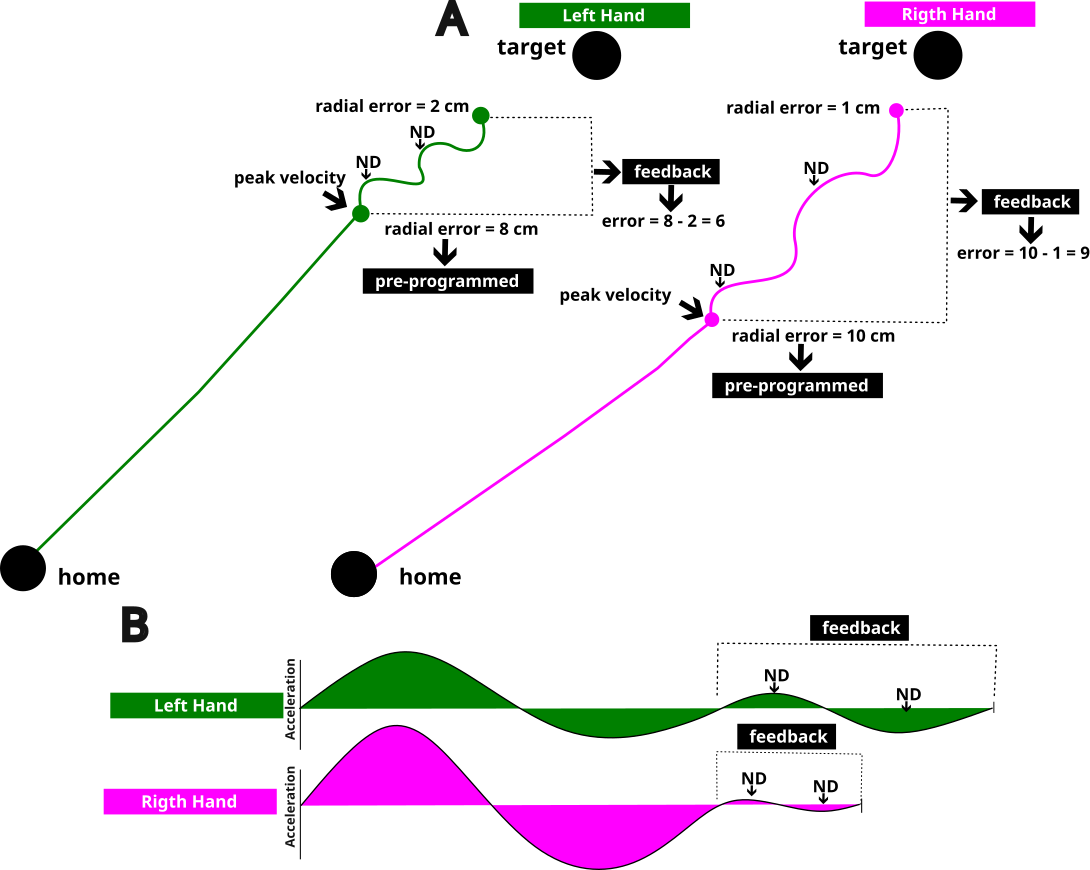
\includegraphics[width=\linewidth]{figures/f1.png}
\caption{Measures of radial error and angle error at peak velocity}
\label{fig1}
\end{figure}


\begin{figure}[p] %h = colocar no mesmo local p = colocar no final
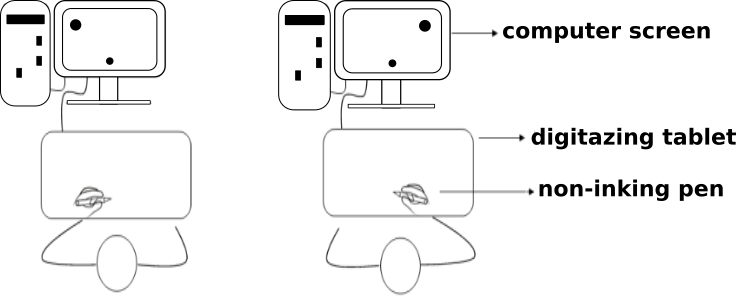
\includegraphics[width=\linewidth]{figures/f2.png}
\caption{Motor task and Apparatus}
\label{fig2}
\end{figure}

\begin{figure}[p] %h = colocar no mesmo local p = colocar no final
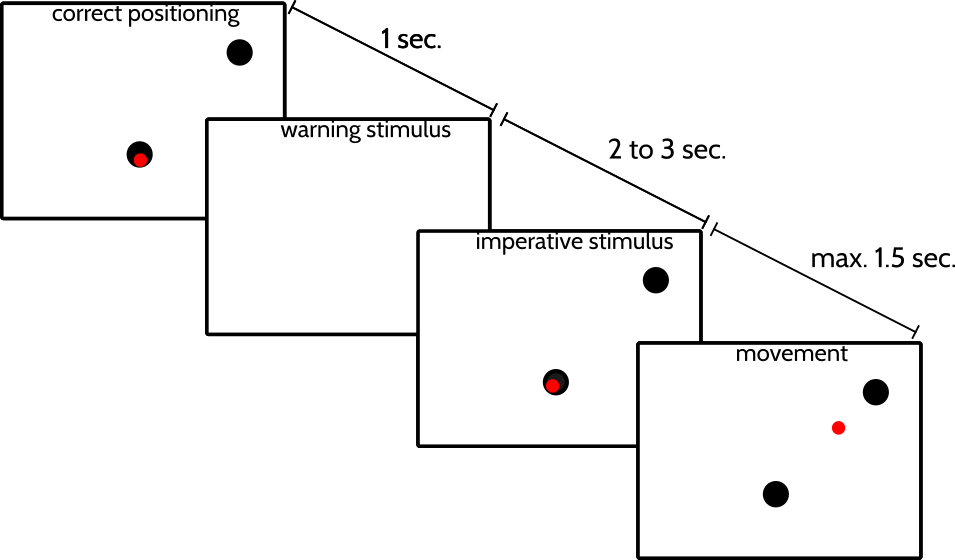
\includegraphics[width=\linewidth]{figures/f3.png}
\caption{Task Scheme}{Red circle = cursor on the computer screen.}
\label{fig3}
\end{figure}


\begin{figure}[p] %h = colocar no mesmo local p = colocar no final
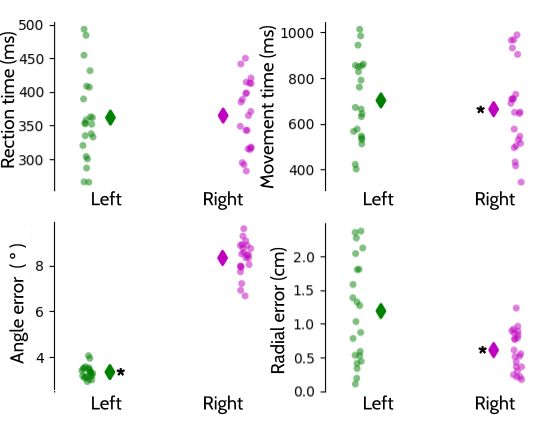
\includegraphics[width=\linewidth]{figures/f4.png}
\caption{Results of reaction time, movement time, radial error, and angle error}{$\diamondsuit$ = mean of hand. $\ocircle$ = individual value of hand. * = difference between hands.}
\label{fig4}
\end{figure}


\begin{figure}[p] %h = colocar no mesmo local p = colocar no final
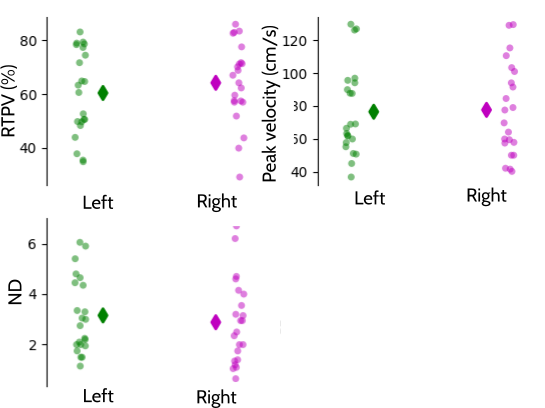
\includegraphics[width=\linewidth]{figures/f5.png}
\caption{Results of relative time to peak velocity, number of discontinuities, and peak velocity}{$\diamondsuit$ = mean of hand. $\ocircle$ = individual value of hand. * = difference between hands. RTPV = relative time to peak velocity. ND = number of discontinuities.}
\label{fig5}
\end{figure} 


\begin{figure}[p] %h = colocar no mesmo local p = colocar no final
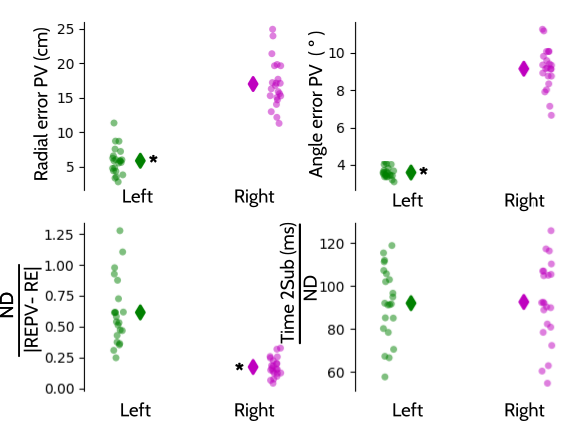
\includegraphics[width=\linewidth]{figures/f6.png}
\caption{Results of radial error at peak velocity, angle error at peak velocity, division of ND by error in the second submovement, and division of time spent in the second submovement by ND}{$\diamondsuit$ = mean of hand. $\ocircle$ = individual value of hand. * = difference between hands. PV = peak velocity. ND = number of discontinuitie. RE = radial error. REPV = radial error in the second submovement. Time2Sub = time spent in the second submovement.}
\label{fig6}
\end{figure} 

\begin{figure}[p] %h = colocar no mesmo local p = colocar no final
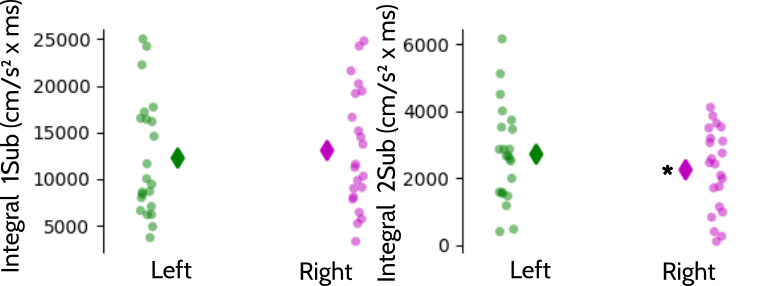
\includegraphics[width=\linewidth]{figures/f7.png}
\caption{Results of integral of absolute acceleration in the first submovement and integral of absolute acceleration in the second submovement}{$\diamondsuit$ = mean of hand. $\ocircle$ = individual value of hand. * = difference between hands.}
\label{fig6}
\end{figure} 


\end{document}
